\sloppy
\section{Daftar Sumber Kode LaTeX / Source}

\begin{figure}[ht]
	\centerline{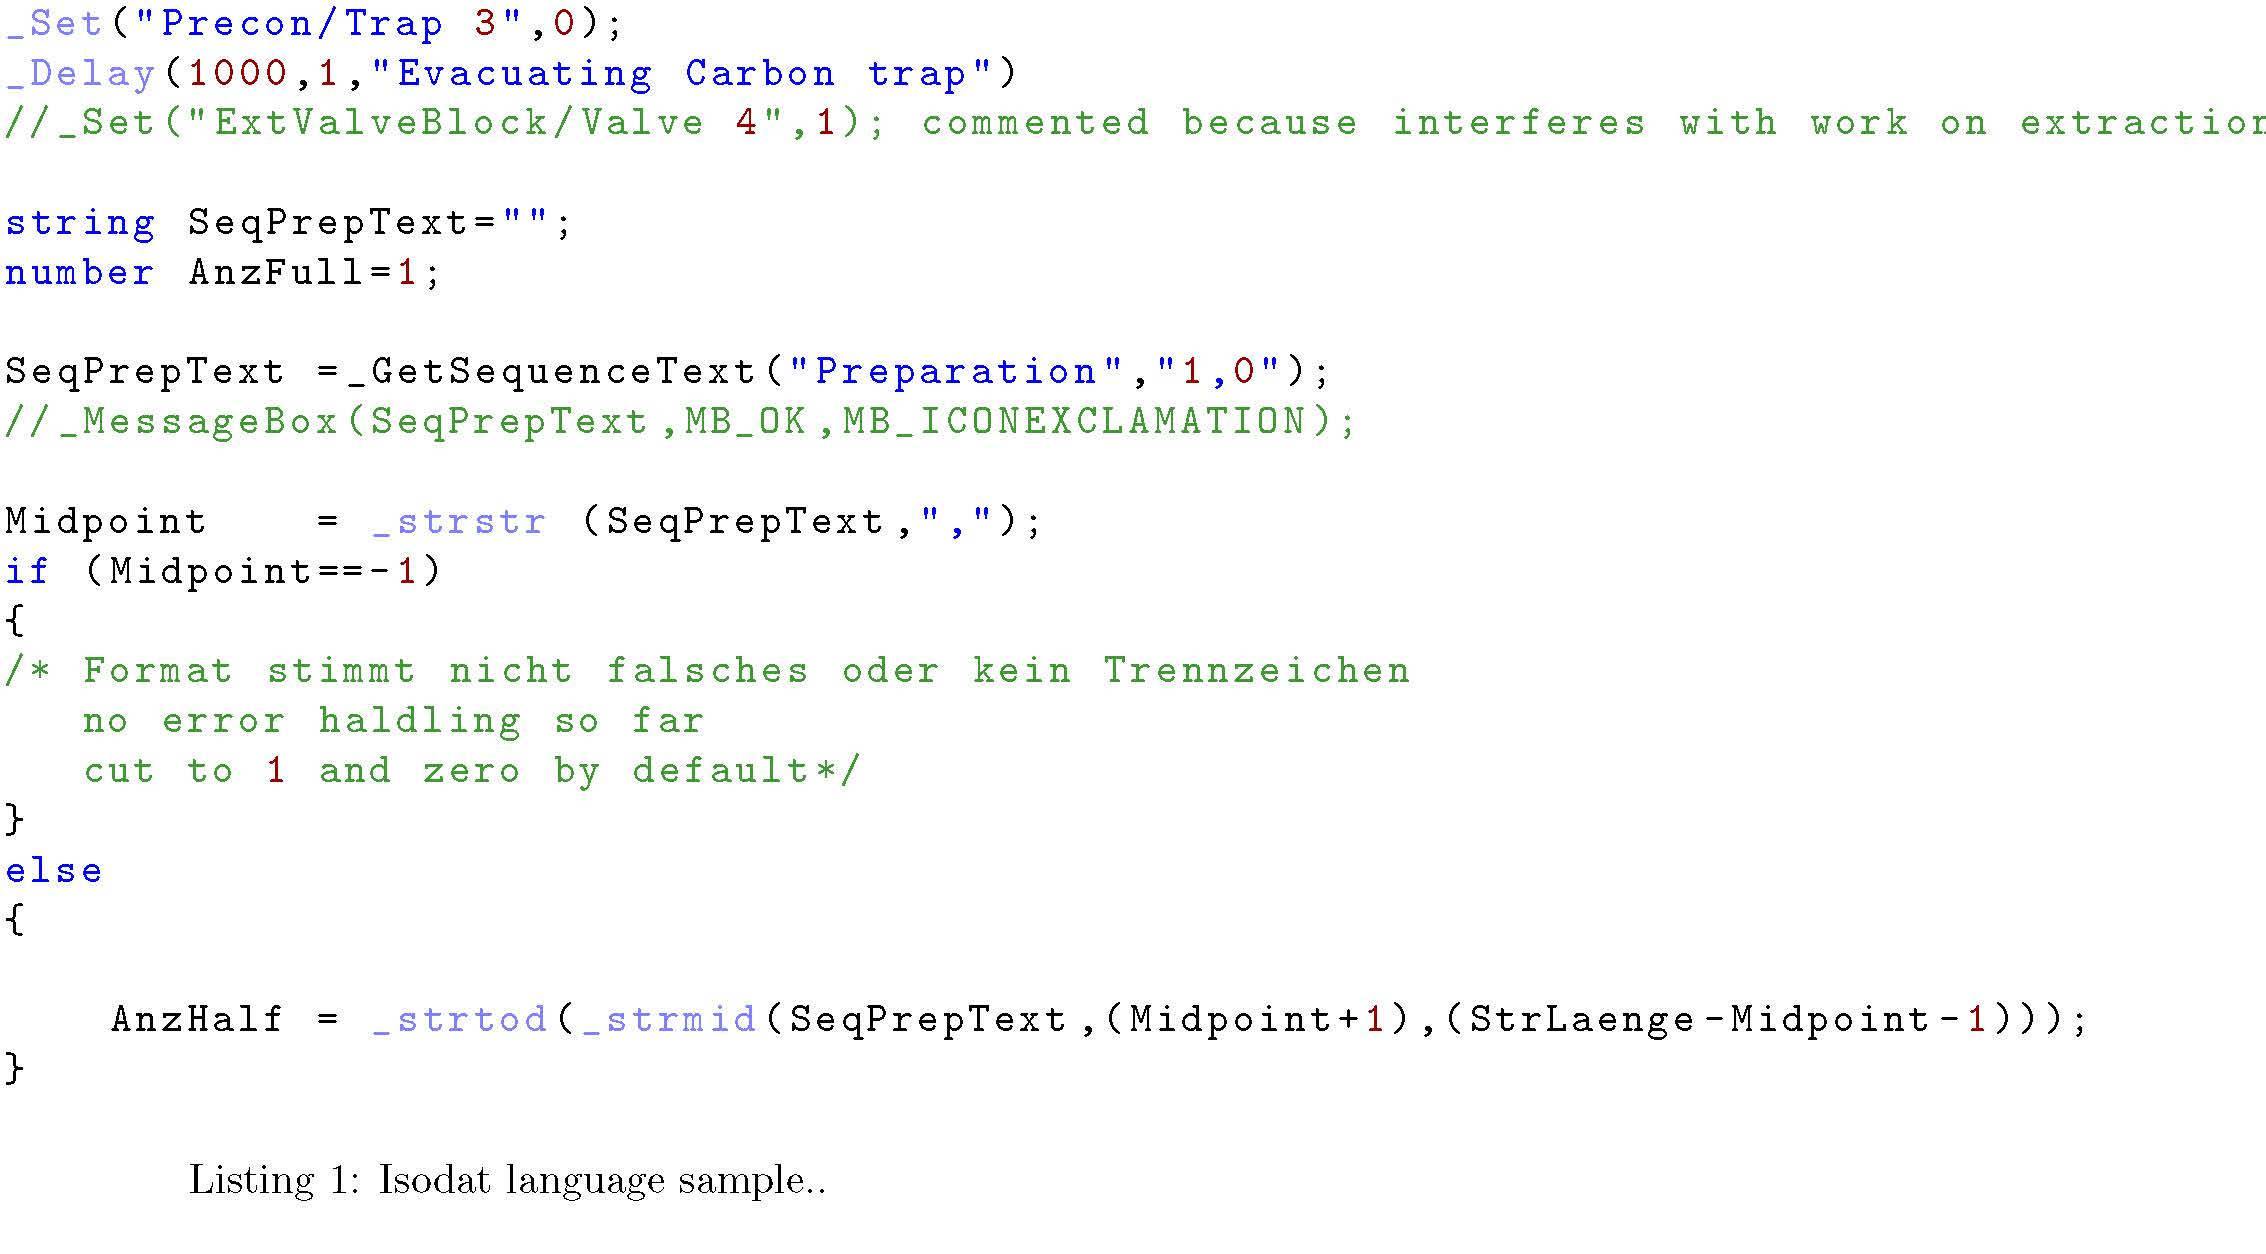
\includegraphics[width=0.50\textwidth]{gambar/contoh1}}
	\caption{Contoh Source code}
	\label{contoh}
\end{figure}

Menggunakan paket daftar \par

Dengan menggunakan daftar paket Anda dapat menambahkan teks yang tidak diformat seperti yang akan Anda lakukan dengan $\textbackslash$begin $ \{ $ verbatim $ \} $ namun tujuan utamanya adalah memasukkan kode sumber dari bahasa pemrograman apa pun ke dalam dokumen Anda. Jika Anda ingin memasukkan pseudocode atau algoritma, Anda mungkin menemukan Algoritma dan Pseudocode berguna juga.\par

Untuk menggunakan paket tersebut, Anda memerlukan:\par

$\textbackslash$ usepackage $ \{ $ listings $ \} $\par

Paket daftar mendukung penyorotan semua bahasa yang paling umum dan sangat mudah disesuaikan. Jika Anda hanya ingin menulis kode dalam dokumen Anda, paket tersebut menyediakan lingkungan lstlisting :\par

$\textbackslash$ begin $ \{ $ lstlisting $ \} $\par

 Letakkan kode anda disini\par

 $\textbackslash$ end $ \{ $ lstlisting $ \} $\par

Kemungkinan lain, itu sangat berguna jika Anda membuat program pada beberapa file dan Anda masih mengeditnya, adalah dengan mengimpor kode dari sumbernya sendiri. Dengan cara ini, jika Anda memodifikasi sumbernya, Anda hanya perlu mengkompilasi ulang kode LaTeX dan dokumen Anda akan diperbarui. Perintahnya adalah:\par

$\textbackslash$ lstinputlisting $ \{ $ source $ \_ $ filename.py $ \} $\par

dalam contoh ada sumber Python, tapi tidak masalah: Anda bisa memasukkan file apapun tapi Anda harus menulis nama file lengkap. Ini akan dianggap teks biasa dan akan disorot sesuai setting Anda, itu berarti tidak mengenali bahasa pemrograman dengan sendirinya. Anda bisa menentukan bahasa sementara menyertakan file dengan perintah berikut:\par

$\textbackslash$ lstinputlisting [language = Python] $ \{ $ source $ \_ $ filename.py $ \} $\par

Anda juga bisa menentukan ruang lingkup untuk file tersebut.\par

$\textbackslash$ lstinputlisting [bahasa = Python, firstline = 37, lastline = 45] $ \{ $ source $ \_ $ filename.py $ \} $\par

Ini sangat berguna jika Anda yakin file tersebut tidak akan berubah (setidaknya sebelum baris yang ditentukan). Anda juga dapat menghilangkan parameter firstline atau lastline : itu berarti semuanya sesuai atau dimulai dari titik ini .\par

Ini adalah contoh dasar untuk beberapa kode Pascal:\par

 $\textbackslash$ documentclass $ \{ $ article $ \} $\par

 $\textbackslash$ usepackage $ \{ $ listings $ \} $ $\%$ Sertakan daftar-paket\par

 $\textbackslash$ begin $ \{ $ document $ \} $\par

 $\textbackslash$ lstset $ \{ $ language = Pascal $ \} $ $\%$ Atur bahasa Anda (Anda dapat mengubah bahasa untuk setiap blok kode secara opsional)\par

 $\textbackslash$ begin $ \{ $ lstlisting $ \} $ [frame = single] $\%$ Mulai blok kode Anda\par

 untuk i: = maxint to 0 do\par

 mulai\par

 $ \{ $ do nothing $ \} $\par

 akhir;\par

 Tulislah ('Case insensitive');\par

 Tulis ('kata kunci Pascal'.);\par

 $\textbackslash$ end $ \{ $ lstlisting $ \} $\par

 $\textbackslash$ end $ \{ $ document $ \} $\par

Bahasa yang didukung \par

Ini mendukung bahasa pemrograman berikut:\par

ABAP 2,4 , ACSL, Ada 4 , Algol 4 , Ant, Assembler 2,4 , Awk 4 , bash, Dasar 2,4 , C $\#$ 5 , C ++ 4 , C 4 , Caml 4 , Clean, Cobol 4 , Comal, csh , Delphi, Eiffel, Elan, erlang, Euforia, Fortran 4 , GCL, Gnuplot, Haskell, HTML, IDL 4 , informasikan, Java 4 , JVMIS, ksh, Lisp 4 , Logo, Lua 2 , buat 4 , Mathematica 1,4 , Matlab, Mercury, MetaPost, Miranda, Mizar, ML, Modelica 3 , Modula-2, MuPAD, NASTRAN, Oberon-2, Tujuan C 5 , OCL 4 , Octave, Oz, Pascal 4 , Perl, PHP, PL / I, Plasm , POV, Prolog, Promela, Python, R, Reduce, Rexx, RSL, Ruby, S 4 , SAS, Scilab, sh, SHELXL, Simula 4 , SQL, tcl 4 , TeX 4 , VBScript, Verilog, VHDL 4 , VRML 4 , XML, XSLT.\par

Bagi beberapa dari mereka, beberapa dialek didukung. Untuk informasi lebih lanjut, lihat dokumentasi yang disertakan dengan paket, harus berada dalam distribusi Anda dengan daftar nama - *. Dvi .\par

Catatan\par

Ini mendukung kode Mathematica hanya jika Anda mengetik dalam format teks biasa. Anda tidak dapat menyertakan file * .NB $\textbackslash$lstinputlisting $ \{ $ ... $ \} $ seperti yang Anda bisa dengan bahasa pemrograman lainnya, namun Mathematica dapat mengekspornya ke sumber LaTeX yang berformat cantik.\par

Spesifikasi dialek adalah wajib untuk bahasa-bahasa ini (misalnya language= $ \{ $ [x86masm]Assembler $ \} $ ).\par

Modelica didukung melalui paket dtsyntax yang tersedia.\par

Untuk bahasa ini, beberapa dialek didukung. C, misalnya, memiliki ANSI, Handel, Objective dan Sharp. Lihat hal. 12 dari manual daftar untuk ikhtisar.\par

Ditetapkan sebagai dialek bahasa lain\par

Pengaturan \par

Anda dapat memodifikasi beberapa parameter yang akan mempengaruhi bagaimana kode ditampilkan. Anda dapat menempatkan kode berikut di manapun dalam dokumen (tidak masalah apakah sebelum atau sesudah $\textbackslash$begin $ \{ $ document $ \} $ ), ubahlah sesuai kebutuhan Anda. Maknanya dijelaskan di samping garis mana saja.\par
\begin{verbatim}
 \ usepackage { listings }
\ usepackage { color }
\ definecolor { mygreen } { rgb } { 0,0.6,0 }
\ definecolor { mygray } { rgb } { 0.5.0.5.0.5 }
\ definecolor { mymauve } { rgb } { 0.58,0,0.82 }
\ lstset { %

\end{verbatim}


~~ backgroundcolor = $\textbackslash$ color $ \{ $ white~$ \} $~, $\%$ pilih warna latar belakang;  Anda harus menambahkan $\textbackslash$ usepackage $ \{ $color$ \} $ or $\textbackslash$ usepackage $ \{ $xcolor$ \} $;  harus datang sebagai argumen terakhir\par

~~ basicstyle = $\textbackslash$ footnotesize , $\%$ ukuran font yang digunakan untuk kode\par

~~ breakatwhitespace = false, $\%$ set jika jeda otomatis seharusnya hanya terjadi di spasi\par

~~ breaklines = true, $\%$ set baris otomatis melanggar\par

~~ captionpos = b, $\%$ set caption-posisi ke bawah\par

~~ commentstyle = $\textbackslash$ color $ \{ $ mygreen $ \} $ , $\%$ style komentar\par

~~ deletekeywords = $ \{ $ ... $ \} $ , $\%$ jika Anda ingin menghapus kata kunci dari bahasa yang diberikan\par

~~ escapeinside = $ \{ $ $\textbackslash$$\%$ * $ \} $ $ \{ $ *) $ \} $ , $\%$ jika Anda ingin menambahkan LaTeX dalam kode Anda\par

~~ extendedchars = true, $\%$ memungkinkan Anda menggunakan karakter non-ASCII;~ untuk pengkodean 8-bit saja, tidak bekerja dengan UTF-8\par

~~ frame = single, $\%$ menambahkan bingkai di sekitar kode\par

~~ keepspaces = true, $\%$ menyimpan spasi di teks, berguna untuk menjaga indentasi kode (mungkin membutuhkan kolom = fleksibel)\par

~~ keywordstyle = $\textbackslash$ color $ \{ $ blue $ \} $ , $\%$ gaya kata kunci\par

~~ bahasa = Octave, $\%$ bahasa kode\par

~~ morekeywords = $ \{ $ *, ... $ \} $ , $\%$ jika Anda ingin menambahkan lebih banyak kata kunci ke himpunan\par

~~ nomor = kiri, $\%$ di mana untuk menempatkan nomor baris;~ nilai yang mungkin adalah (none, left, right)\par

~~ numberep = 5pt, $\%$ seberapa jauh garis-angka dari kode\par

~~ numbertyle = $\textbackslash$ tiny $\textbackslash$ color $ \{ $ mygray $ \} $ , $\%$ style yang digunakan untuk line-numbers\par

~~ rulecolor = $\textbackslash$ color $ \{ $ black $ \} $ , $\%$ jika tidak disetel, warna bingkai dapat berubah pada garis-jeda dalam teks tidak-hitam (misalnya komentar (hijau di sini))\par

~~ showpaces = false, $\%$ show spaces dimana-mana menambahkan garis bawah tertentu;~ itu menimpa 'showstringspaces'\par

~~ showstringspaces = false, $\%$ menggarisbawahi ruang dalam string saja\par

~~ showtabs = false, $\%$ tampilkan tab dalam string yang menambahkan garis bawah tertentu\par

~~~stepnumber = 2, $\%$ langkah antara dua line-numbers.  Jika 1, setiap baris akan diberi nomor\par

~~ stringstyle = $\textbackslash$ color $ \{ $ mymauve $ \} $ , $\%$ string literal style\par

~~ tabsize = 2, $\%$ set tabsize default menjadi 2 spasi\par

~~ title = $\textbackslash$ lstname $\%$ tampilkan nama file yang disertakan dengan $\textbackslash$ lstinputlisting;~ juga mencoba judul dan bukan judul\par

 $ \} $\par

Escapeinside\par

Garis pelarian membutuhkan penjelasan. Pilihan escapeinside= $ \{ $ A $ \} $$ \{ $ B $ \} $ akan menentukan pembatas untuk lolos ke kode LaTeX, yaitu semua kode antara string "A" dan "B" akan diuraikan sebagai LaTeX dari daftar gaya saat ini. Pada contoh di atas, komentar untuk Octave dimulai dengan $\%$ , dan akan dicetak dalam dokumen kecuali jika dimulai dengan $\%$* , dalam hal ini mereka dibaca sebagai LaTeX (dengan semua perintah LaTeX terpenuhi) sampai ditutup dengan yang lain *) . Jika Anda menambahkan paragraf di atas, berikut ini dapat digunakan untuk mengubah pengaturan dalam kode:\par

$\textbackslash$ lstset $ \{ $ language = C, caption = $ \{ $ Teks Keterangan Deskriptif $ \} $ , label = DeskriptifLabel $ \} $\par

Ada lebih banyak pilihan, periksa dokumentasi resmi.\par

Definisi gaya \par

Paket ini memungkinkan Anda menentukan gaya, yaitu profil yang menentukan satu set pengaturan.\par

Contoh\par

\begin{enumerate}
	\item lstdefinestyle  customc 
	\item belowcaptionskip = 1 \ baselineskip ,
	\item	breaklines = true,
	\item	frame = L,
	\item	xleftmargin = \ parindent ,
	\item	bahasa = C,
	\item	showstringspaces = false,
	\item	basicstyle = \ footnotesize \ ttfamily ,
	\item	keywordstyle = \ bfseries \ color  green! 40! black  ,
	\item	commentstyle = \ itshape \ color  ungu! 40! hitam  ,
	\item	identifierstyle = \ color  blue  ,
	\item	stringstyle = \ color  orange  ,
	 \item   lstdefinestyle  customasm 
	\item	belowcaptionskip = 1 \ baselineskip ,
	\item	frame = L,
	\item	xleftmargin = \ parindent ,
	\item	bahasa = [x86masm] Assembler,
	\item	basicstyle = \ footnotesize \ ttfamily ,
	\item	commentstyle = \ itshape \ color  ungu! 40! hitam  ,
	 \item   lstset  escapechar = @, style = customc 
\end{enumerate}



Dalam contoh kita, kita hanya menetapkan dua pilihan secara global: gaya default dan karakter escape. Pemakaian:\par

 $\setminus$ begin $ \{ $ lstlisting $ \} $\par

 $\#$include <stdio.h>\par

 $\#$define N 10\par

 / * Blokir\par

 * komentar * /\par

 int main ()\par

 $ \{ $\par

~~~~ int i ;\par

~~~~ // Baris komentar\par

~~~~ menempatkan ( "Halo dunia!" );\par

~~~ \par

~~~~ untuk ( i = 0 ; i < N ; i ++ )\par

~~~~ $ \{ $\par

~~~~~~~~ menempatkan ( "LaTeX juga bagus untuk pemrogram!" );\par

~~~~ $ \} $\par

~~~~ kembali 0 ;\par

 $ \} $\par

 $\textbackslash$ end $ \{ $ lstlisting $ \} $\par

 $\textbackslash$ lstinputlisting [ caption = Scheduler ,~style = customc ] $ \{ $ halo .  c $ \} $\par

Mengotomatiskan file inclusion \par

Jika Anda memiliki banyak file sumber yang ingin Anda sertakan, Anda mungkin mendapati diri Anda melakukan hal yang sama berulang-ulang. Di sinilah makro menunjukkan kekuatan sesungguhnya mereka.\par

 $\textbackslash$ newcommand $ \{ $ $\textbackslash$ includecode $ \} $ [2] [c] $ \{ $ $\textbackslash$ lstinputlisting [caption = $\#$ 2, escapechar =, style = custom $\#$ 1] $ \{ $ $\#$ 2 $ \} $ <! ----> $ \} $\par

 $\%$ ...\par

 $\textbackslash$ includecode $ \{ $ sched.c $ \} $\par

 $\textbackslash$ includecode [asm] $ \{ $ sched.s $ \} $\par

 $\%$ ...\par

 $\textbackslash$ lstlistoflistings\par

Dalam contoh ini, kita membuat satu perintah untuk memudahkan penyertaan kode sumber. Kami menetapkan gaya default menjadi customc . Semua daftar akan memiliki nama mereka sebagai caption: kita tidak perlu menuliskan nama file dua kali terima kasih kepada makro. Akhirnya kami daftar semua daftar dengan perintah ini dari daftar paket.\par

Lihat Makro untuk lebih jelasnya.\par

Encoding issue \par

Secara default, daftar tidak mendukung pengkodean multi-byte untuk kode sumber. Pilihan extendedchar hanya bekerja untuk pengkodean 8-bit seperti latin1.\par

Untuk menangani UTF-8, Anda harus memberi tahu cantuman bagaimana menafsirkan karakter khusus dengan menentukannya seperti itu\par

 $\textbackslash$ lstset $ \{ $ melek huruf =\par

~~ $ \{ $$ \{ $ $ \} $ $ \} $ $ \{ $$ \{ $ $\textbackslash$ ' $ \} $$ \} $ 1 $ \{ $ í $ \} $ $ \{ $$ \{ $ $\textbackslash$' i $ \} $$ \} $ 1 $ \{ $ ó $ \} $ $ \{ $$ \{ $ $\textbackslash$ ' o $ \} $$ \} $ 1 $ \{ $ ú $ \} $ $ \{ $$ \{ $ $\textbackslash$ ' u $ \} $$ \} $ 1\par

~~ $ \{ $$ \{ $ $ \} $$ \} $ $ \{ $$ \{ $ $\textbackslash$ ' A $ \} $$ \} $ 1 $ \{ $ É $ \} $ $ \{ $$ \{ $ $\textbackslash$' E $ \} $$ \} $ 1 $ \{ $ Í $ \} $ $ \{ $$ \{ $ $\textbackslash$ ' I $ \} $$ \} $ 1 $ \{ $ Ó $ \} $ $ \{ $$ \{ $ $\textbackslash$' O $ \} $$ \} $ 1 $ \{ $ Ú $ \} $ $ \{ $$ \{ $ $\textbackslash$ ' U $ \} $$ \} $ 1\par

~~ $ \{ $ à $ \} $ $ \{ $$ \{ $ $\textbackslash$ ` a $ \} $$ \} $ 1 $ \{ $ è $ \} $ $ \{ $$ \{ $ $\textbackslash$` e $ \} $$ \} $ 1 $ \{ $ ì $ \} $ $ \{ $$ \{ $ $\textbackslash$ ` i $ \} $$ \} $ 1 $ \{ $ ò $ \} $ $ \{ $$ \{ $ $\textbackslash$` o $ \} $$ \} $ 1 $ \{ $ ù $ \} $ $ \{ $$ \{ $ $\textbackslash$ ` u $ \} $$ \} $ 1\par

~~ $ \{ $$ \{ $ $ \} $$ \} $ $ \{ $$ \{ $ $\textbackslash$ $\textbackslash$ $ \} $$ \} $ 1 $ \{ $ È $ \} $ $ \{ $$ \{ $ $\textbackslash$ ' I $ \} $$ \} $ 1 $ \{ $ Ò $ \} $ $ \{ $$ \{ $ $\textbackslash$ ` O $ \} $$ \} $ 1 $ \{ $ Ù $ \} $ $ \{ $$ \{ $ $\textbackslash$ ` U $ \} $$ \} $ 1\par

~~ $ \{ $$ \{ $ $ \} $ $ \} $ $ \{ $$ \{ $ $\textbackslash$ " e $ \} $$ \} $ 1 $ \{ $ ò $ \} $ $ \{ $$ \{ $ $\textbackslash$" i $ \} $$ \} $ 1 $ \{ $ ö $ \} $ $ \{ $$ \{ $ $\textbackslash$ " o $ \} $$ \} $ 1 $ \{ $ ü $ \} $ $ \{ $$ \{ $ $\textbackslash$ " u $ \} $$ \} $ 1\par

~~ $ \{ $ $ \} $ $ \{ $$ \{ $ $\textbackslash$ " A $ \} $$ \} $ 1 $ \{ $ Ë $ \} $ $ \{ $$ \{ $ $\textbackslash$" E $ \} $$ \} $ 1 $ \{ $ Ï $ \} $ $ \{ $$ \{ $ $\textbackslash$ " I $ \} $$ \} $ 1 $ \{ $ Ö $ \} $ $ \{ $$ \{ $ $\textbackslash$" O $ \} $$ \} $ 1 $ \{ $ Ü $ \} $ $ \{ $$ \{ $ $\textbackslash$ " U $ \} $$ \} $ 1\par

~~ $ \{ $ $ \} $ $ \{ $$ \{ $ $\textbackslash$ $ \string^ $ a $ \} $$ \} $ 1 $ \{ $ ê $ \} $ $ \{ $$ \{ $ $\textbackslash$ $ \string^ $ e $ \} $$ \} $ 1 $ \{ $ î $ \} $ $ \{ $$ \{ $ $\textbackslash$ $ \string^ $ i $ \} $$ \} $ 1 $ \{ $ ô $ \} $ $ \{ $$ \{ $ $\textbackslash$ $ \string^ $ o $ \} $$ \} $ 1 $ \{ $ û $ \} $ $ \{ $$ \{ $ $\textbackslash$ $ \string^ $ u $ \} $$ \} $ 1\par

~~ $ \{ $$ \{ $ $ \} $$ \} $ $ \{ $$ \{ $ $ \string^ $ $ \} $$ \} $ $ \{ $$ \{ $ $ \} $$ \} $$ \} $ $ \{ $$ \{ $ $\textbackslash$ $\textbackslash$ $ \} $$ \} $ $ \{ $$ \{ $$ \} $$ \} $$ \} $ $ \{ $$ \{ $ $\textbackslash$ $\textbackslash$ $ \} $$ \} $ $ \{ $$ \{ $ $ \} $ $\textbackslash$ $ \string^ $ I $ \} $$ \} $ 1 $ \{ $ Ô $ \} $ $ \{ $$ \{ $ $\textbackslash$ $ \string^ $ O $ \} $$ \} $ 1 $ \{ $ Û $ \} $ $ \{ $$ \{ $ $\textbackslash$ $ \string^ $ U $ \} $$ \} $ 1\par

~~ $ \{ $ $ \} $ $ \{ $$ \{ $ $\textbackslash$ oe $ \} $$ \} $ 1 $ \{ $ Œ $ \} $ $ \{ $$ \{ $ $\textbackslash$ OE $ \} $$ \} $ 1 $ \{ $ æ $ \} $ $ \{ $$ \{ $ $\textbackslash$ ae $ \} $$ \} $ 1 $ \{ $ Æ $ \} $ $ \{ $$ \{ $ $\textbackslash$ AE $ \} $$ \} $ 1 $ \{ $ ß $ \} $ $ \{ $$ \{ $ $\textbackslash$ ss $ \} $$ \} $ 1\par

~~ $ \{ $ ű $ \} $ $ \{ $$ \{ $ $\textbackslash$ H $ \{ $ u $ \} $$ \} $$ \} $ 1 $ \{ $ Ű $ \} $ $ \{ $$ \{ $ $\textbackslash$ H $ \{ $ U $ \} $$ \} $$ \} $ 1 $ \{ $ ő $ \} $ $ \{ $$ \{ $ $\textbackslash$ H $ \{ $ o $ \} $$ \} $$ \} $ 1 $ \{ $ Ő $ \} $ $ \{ $$ \{ $ $\textbackslash$ H $ \{ $ O $ \} $$ \} $ $ \} $ 1\par

~~ $ \{ $ ç $ \} $ $ \{ $$ \{ $ c $ \} $$ \} $ 1 $ \{ $ Ç $ \} $ $ \{ $$ \{ $ c $ \} $$ \} $ 1 $ \{ $ ø $ \} $ $ \{ $$ \{ $ $\textbackslash$ o $ \} $$ \} $ 1 $ \{ $ å $ \} $ $ \{ $$ \{ $ $\textbackslash$ $\textbackslash$ $ \} $$ \} $ 1 $ \{ $ Å $ \} $ $ \{ $$ \{ $ $\textbackslash$ r A $ \} $$ \} $ 1\par

~~ $ \{ $ € $ \} $ $ \{ $$ \{ $ $\textbackslash$ euro $ \} $$ \} $ 1 $ \{ $ £ $ \} $ $ \{ $$ \{ $ $\textbackslash$ pound $ \} $$ \} $ 1 $ \{ $ « $ \} $ $ \{ $$ \{ $ $\textbackslash$ guillemotleft $ \} $$ \} $ 1\par

~~ $ \{ $ $ \} $$ \} $ $ \{ $$ \{ $ $\textbackslash$ Guillemotright $ \} $$ \} $ 1 $ \{ $ ñ $ \} $ $ \{ $$ \{ $ $\textbackslash$ $ \sim $ n $ \} $$ \} $ 1 $ \{ $ Ñ $ \} $ $ \{ $$ \{ $ $\textbackslash$ $ \sim $ N $ \} $$ \} $ 1 $ \{ $ ¿ $ \} $ $ \{ $$ \{ $ ? ` $ \} $$ \} $ 1\par

 $ \} $\par

Tabel di atas akan mencakup sebagian besar karakter dalam bahasa latin. Untuk penjelasan lebih rinci tentang penggunaan bagian cek pilihan literate 6.4 di Dokumentasi Listing .\par

Kemungkinan lain adalah mengganti $\textbackslash$usepackage $ \{ $ listings $ \} $ (dalam basa-basi) dengan $\textbackslash$usepackage $ \{ $ listingsutf8 $ \} $ , tapi ini hanya akan bekerja untuk $\textbackslash$lstinputlisting $ \{ $ ... $ \} $ .\par

Menyesuaikan caption \par

Anda dapat memiliki caption mewah (atau judul) untuk cantuman Anda menggunakan paket teks . Berikut adalah contoh untuk daftar .\par

 $\textbackslash$ usepackage $ \{ $ caption $ \} $\par

 $\textbackslash$ usepackage $ \{ $ listings $ \} $\par

 $\textbackslash$ DeclareCaptionFont $ \{ $ white $ \} $ $ \{ $ $\textbackslash$ color $ \{ $ white $ \} $ $ \} $\par

 $\textbackslash$ DeclareCaptionFormat $ \{ $ listing $ \} $ $ \{ $\par

~~ $\textbackslash$ colorbox [cmyk] $ \{ $ 0.43, 0.35, 0.35.0.01 $ \} $ $ \{ $\par

~~~~ $\textbackslash$ parbox $ \{ $ $\textbackslash$ textwidth $ \} $ $ \{ $ $\textbackslash$ hspace $ \{ $ 15pt $ \} $ $\#$ 1 $\#$ 2 $\#$ 3 $ \} $\par

~~ $ \} $\par

 $ \} $\par

 $\textbackslash$ capionsetup [lstlisting] $ \{ $ format = daftar, labelfont = putih, textfont = putih, singlelinecheck = false, margin = 0pt, font = $ \{ $ bf, footnotesize $ \} $ $ \} $\par

 $\%$ ...\par

 $\textbackslash$ lstinputlisting [caption = My caption] $ \{ $ sourcefile.lang $ \} $\par

Paket yang dicetak \par

dicetak adalah alternatif untuk daftar yang telah menjadi populer. Menggunakan Python eksternal perpustakaan Pygments untuk menyoroti kode, yang pada November 2014 menawarkan lebih dari 300 bahasa dan format teks yang didukung.\par

Karena paket bergantung pada kode Python eksternal, penyiapan memerlukan beberapa langkah lebih banyak daripada paket LaTeX biasa, jadi mohon lihat repo GitHub dan manualnya .\par

Catatan\par

Ini mendukung kode Mathematica hanya jika Anda mengetik dalam format teks biasa. Anda tidak dapat menyertakan file * .NB $\textbackslash$lstinputlisting $ \{ $ ... $ \} $ seperti yang Anda bisa dengan bahasa pemrograman lainnya, namun Mathematica dapat mengekspornya ke sumber LaTeX yang berformat cantik.\par

Spesifikasi dialek adalah wajib untuk bahasa-bahasa ini (misalnya language= $ \{ $ [x86masm]Assembler $ \} $ ).\par

Modelica didukung melalui paket dtsyntax yang tersedia.\par

Untuk bahasa ini, beberapa dialek didukung. C, misalnya, memiliki ANSI, Handel, Objective dan Sharp. Lihat hal. 12 dari manual daftar untuk ikhtisar.\par

Ditetapkan sebagai dialek bahasa lain\par

Pengaturan \par

Anda dapat memodifikasi beberapa parameter yang akan mempengaruhi bagaimana kode ditampilkan. Anda dapat menempatkan kode berikut di manapun dalam dokumen (tidak masalah apakah sebelum atau sesudah $\textbackslash$begin $ \{ $ document $ \} $ ), ubahlah sesuai kebutuhan Anda. Maknanya dijelaskan di samping garis mana saja.\par

 $\textbackslash$ usepackage $ \{ $ listings $ \} $\par

 $\textbackslash$ usepackage $ \{ $ color $ \} $\par

 $\textbackslash$ definecolor $ \{ $ mygreen $ \} $ $ \{ $ rgb $ \} $ $ \{ $ 0,0.6,0 $ \} $\par

 $\textbackslash$ definecolor $ \{ $ mygray $ \} $ $ \{ $ rgb $ \} $ $ \{ $ 0.5.0.5.0.5 $ \} $\par

 $\textbackslash$ definecolor $ \{ $ mymauve $ \} $ $ \{ $ rgb $ \} $ $ \{ $ 0.58,0,0.82 $ \} $\par

 $\textbackslash$ lstset $ \{ $ $\%$\par

~~ backgroundcolor = $\textbackslash$ color $ \{ $ white~$ \} $~, $\%$ pilih warna latar belakang;  Anda harus menambahkan $\textbackslash$ usepackage $ \{ $color$ \} $ or $\textbackslash$ usepackage $ \{ $xcolor$ \} $;  harus datang sebagai argumen terakhir\par

~~ basicstyle = $\textbackslash$ footnotesize , $\%$ ukuran font yang digunakan untuk kode\par

~~ breakatwhitespace = false, $\%$ set jika jeda otomatis seharusnya hanya terjadi di spasi\par

~~ breaklines = true, $\%$ set baris otomatis melanggar\par

~~ captionpos = b, $\%$ set caption-posisi ke bawah\par

~~ commentstyle = $\textbackslash$ color $ \{ $ mygreen $ \} $ , $\%$ style komentar\par

~~ deletekeywords = $ \{ $ ... $ \} $ , $\%$ jika Anda ingin menghapus kata kunci dari bahasa yang diberikan\par

~~ escapeinside = $ \{ $ $\textbackslash$$\%$ * $ \} $ $ \{ $ *) $ \} $ , $\%$ jika Anda ingin menambahkan LaTeX dalam kode Anda\par

~~ extendedchars = true, $\%$ memungkinkan Anda menggunakan karakter non-ASCII;~ untuk pengkodean 8-bit saja, tidak bekerja dengan UTF-8\par

~~ frame = single, $\%$ menambahkan bingkai di sekitar kode\par

~~ keepspaces = true, $\%$ menyimpan spasi di teks, berguna untuk menjaga indentasi kode (mungkin membutuhkan kolom = fleksibel)\par

~~ keywordstyle = $\textbackslash$ color $ \{ $ blue $ \} $ , $\%$ gaya kata kunci\par

~~ bahasa = Octave, $\%$ bahasa kode\par

~~ morekeywords = $ \{ $ *, ... $ \} $ , $\%$ jika Anda ingin menambahkan lebih banyak kata kunci ke himpunan\par

~~ nomor = kiri, $\%$ di mana untuk menempatkan nomor baris;~ nilai yang mungkin adalah (none, left, right)\par

~~ numberep = 5pt, $\%$ seberapa jauh garis-angka dari kode\par

~~ numbertyle = $\textbackslash$ tiny $\textbackslash$ color $ \{ $ mygray $ \} $ , $\%$ style yang digunakan untuk line-numbers\par

~~ rulecolor = $\textbackslash$ color $ \{ $ black $ \} $ , $\%$ jika tidak disetel, warna bingkai dapat berubah pada garis-jeda dalam teks tidak-hitam (misalnya komentar (hijau di sini))\par

~~ showpaces = false, $\%$ show spaces dimana-mana menambahkan garis bawah tertentu;~ itu menimpa 'showstringspaces'\par

~~ showstringspaces = false, $\%$ menggarisbawahi ruang dalam string saja\par

~~ showtabs = false, $\%$ tampilkan tab dalam string yang menambahkan garis bawah tertentu\par

~~~stepnumber = 2, $\%$ langkah antara dua line-numbers.  Jika 1, setiap baris akan diberi nomor\par

~~ stringstyle = $\textbackslash$ color $ \{ $ mymauve $ \} $ , $\%$ string literal style\par

~~ tabsize = 2, $\%$ set tabsize default menjadi 2 spasi\par

~~ title = $\textbackslash$ lstname $\%$ tampilkan nama file yang disertakan dengan $\textbackslash$ lstinputlisting;~ juga mencoba judul dan bukan judul\par

 $ \} $\par

Kemungkinan lain adalah mengganti $\textbackslash$usepackage $ \{ $ listings $ \} $ (dalam basa-basi) dengan $\textbackslash$usepackage $ \{ $ listingsutf8 $ \} $ , tapi ini hanya akan bekerja untuk $\textbackslash$lstinputlisting $ \{ $ ... $ \} $ .\par

Menyesuaikan caption \par

Anda dapat memiliki caption mewah (atau judul) untuk cantuman Anda menggunakan paket teks . Berikut adalah contoh untuk daftar .\par

 $\textbackslash$ usepackage $ \{ $ caption $ \} $\par

 $\textbackslash$ usepackage $ \{ $ listings $ \} $\par

 $\textbackslash$ DeclareCaptionFont $ \{ $ white $ \} $ $ \{ $ $\textbackslash$ color $ \{ $ white $ \} $ $ \} $\par

 $\textbackslash$ DeclareCaptionFormat $ \{ $ listing $ \} $ $ \{ $\par

~~ $\textbackslash$ colorbox [cmyk] $ \{ $ 0.43, 0.35, 0.35.0.01 $ \} $ $ \{ $\par

~~~~ $\textbackslash$ parbox $ \{ $ $\textbackslash$ textwidth $ \} $ $ \{ $ $\textbackslash$ hspace $ \{ $ 15pt $ \} $ $\#$ 1 $\#$ 2 $\#$ 3 $ \} $\par

~~ $ \} $\par

 $ \} $\par

 $\textbackslash$ capionsetup [lstlisting] $ \{ $ format = daftar, labelfont = putih, textfont = putih, singlelinecheck = false, margin = 0pt, font = $ \{ $ bf, footnotesize $ \} $ $ \} $\par

 $\%$ ...\par

 $\textbackslash$ lstinputlisting [caption = My caption] $ \{ $ sourcefile.lang $ \} $\par
 
 \noindent
 Dalam contoh kita, kita hanya menetapkan dua pilihan secara global: gaya default dan karakter escape. Pemakaian: \par
 
 \begin{verbatim}
\ begin { lstlisting }
#include <stdio.h>
#define N 10
/ * Blokir
* komentar * /

int main ()
{
int i ;

// Baris komentar
menempatkan ( "Halo dunia!" );

untuk ( i = 0 ; i < N ; i ++ )
{
menempatkan ( "LaTeX juga bagus untuk pemrogram!" );
}

kembali 0 ;
}
\ end { lstlisting }

\ lstinputlisting [ caption = Scheduler , style = customc ] { halo .  c }
Bagian C akan dicetak sebagai :
 \end{verbatim}
 
\begin{figure}[ht]
	\centerline{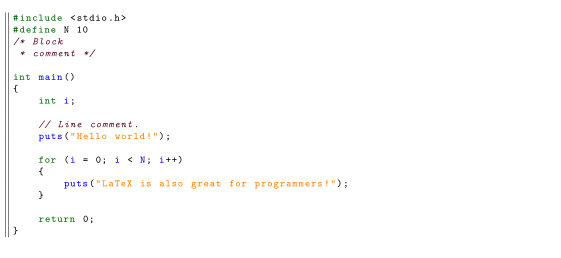
\includegraphics[width=0.50\textwidth]{gambar/contoh3}}
	\caption{Contoh Penggambaran}
	\label{contoh3}
\end{figure}